\section{ХОД РАБОТЫ}

\subsection{Постановка задачи}

В ходе данной лабораторной работы требуется реализовать обучение
персептрона, в результате которого программа, написанная на языке Пролог,
будет корректно распознавать букву <<Я>>.

\subsection{Определение интерфейса программы}

Для решения задачи на языке Пролог необходимо перейти от рукописного
представления символов (например, буквы <<Я>>) к некоторому набору данных.
Определим этот переход следующим образом: для рукописного ввода символа
выделим область, состоящую из $36$ квадратных подобластей.
Будем преобразовывать рукописное представление символа в набор данных по такому
правилу: если подобласть $x_{ij}$ в результате начертания символа оказалось пустой,
то принимаем элемент $x_{ij}$ равным нулю, иначе --- единице.
Пример перехода от рукописного ввода буквы <<Я>> к массиву
данных приведен на рисунке~\ref{fig:symbol_to_matrix}.
\begin{figure}[h!]
  \centering
  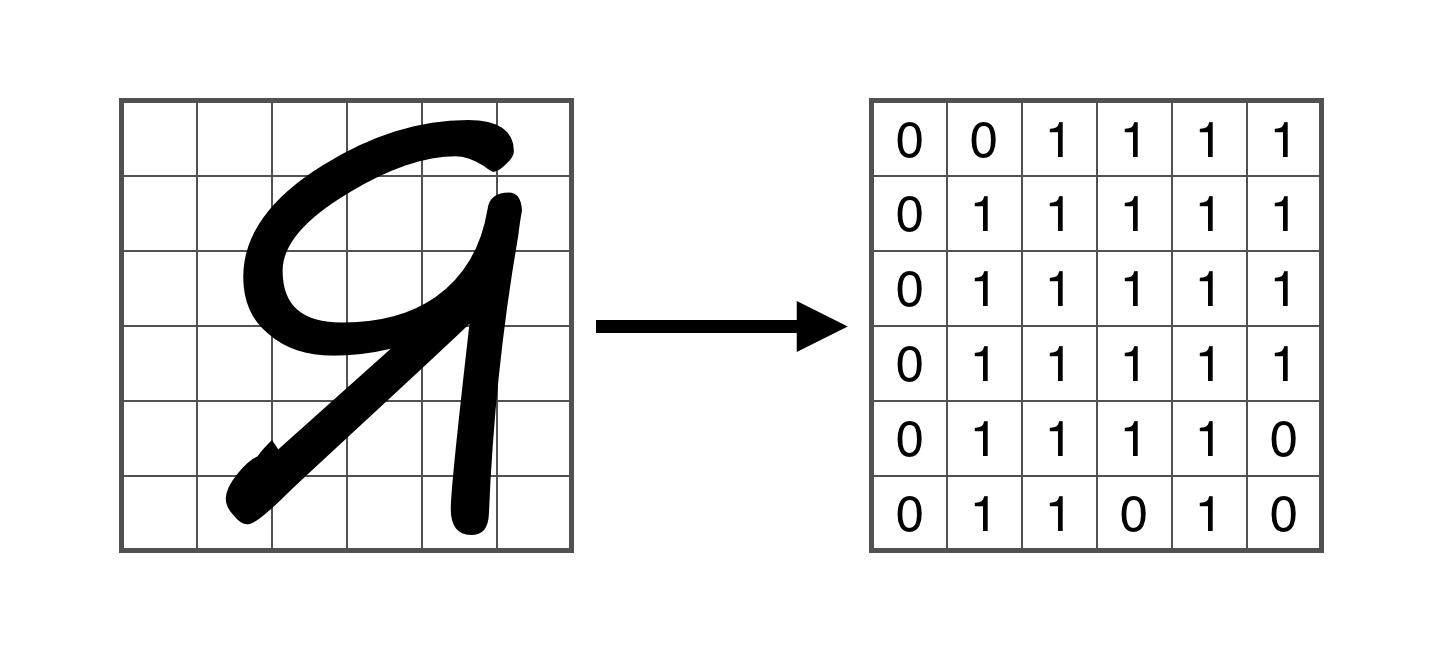
\includegraphics[width=150mm]{img/symbol_to_matrix}
  \caption{Пример перехода от рукописного ввода к массиву данных}
  \label{fig:symbol_to_matrix}
\end{figure}

Таким образом, в качестве сигналов $X =( x_{ij} )$ на вход персептрона
будут подаваться значения $0$ или $1$.


\subsection{Определение исходных данных для персептрона}

Определим начальные значения коэффициентов $a_0$ и $a_i$.
\begin{equation*}
  a_i = 2 \: x_i^E, \hspace{3mm} a_0 = - \sum_{i=1}^{n} (x_i^E)^2, \hspace{3mm} i = \overline{1,n}, \: n=36,
\end{equation*}
где $x_i^E$ --- элементы эталонного объекта, равного:
\[
  \begin{array}{lc}
    X^E = 
    \left(
      \begin{matrix}
        0 \: 0 \: 1 \: 1 \: 1 \: 1 \\
        0 \: 1 \: 1 \: 0 \: 1 \: 1 \\
        0 \: 1 \: 0 \: 0 \: 1 \: 1 \\
        0 \: 1 \: 1 \: 1 \: 1 \: 1 \\
        0 \: 0 \: 1 \: 1 \: 1 \: 0 \\
        0 \: 1 \: 1 \: 0 \: 1 \: 0
      \end{matrix}
    \right).
  \end{array}
\]

Значит, коэффициенты $a_0$ и $a_i$ примут начальные значения:
\begin{align*}
  a_0 = -18, \hspace{3mm}
  \begin{array}{lc}
    A = 
    \left(
      \begin{matrix}
        0 \: 0 \: 2 \: 2 \: 2 \: 2 \\
        0 \: 2 \: 2 \: 0 \: 2 \: 2 \\
        0 \: 2 \: 0 \: 0 \: 2 \: 2 \\
        0 \: 2 \: 2 \: 2 \: 2 \: 2 \\
        0 \: 0 \: 2 \: 2 \: 2 \: 0 \\
        0 \: 2 \: 2 \: 0 \: 2 \: 0
      \end{matrix}
    \right).
  \end{array}
\end{align*}


\newpage
\subsection{Процесс обучения персептрона}

Обучим персептрон, используя следующий алгоритм действий:
\begin{enumerate}
  \item Подставляем полученные коэффициенты $a_0, a_i$ в формулу~\eqref{eq:Y},
  значения $x_i$ берём из обучающей выборки.
  \item Если значение Y больше нуля, значит персептрон распознал символ <<Я>>.
  Если значения сигналов обучающей выборки определяют букву <<Я>>,
  то система ведёт себя корректно, можно переходить к следующей итерации обучения. 
  Иначе необходимо выполнить пересчёт коэффициентов $a_i$:
  \begin{align*}
    a_i &= a_i - x_i, \: a_0 = a_0 - C, \: \text{если выборка } X \text{ определяет символ <<Я>>}, \\
    a_i &= a_i + x_i, \: a_0 = a_0 + C, \: \text{иначе}.
  \end{align*}
  После пересчёта коэффициентов $a_i$ процесс обучения начинается сначала.
\end{enumerate}

Результат работы программы приведен на рисунке~\ref{fig:results}.

\begin{figure}[h!]
  \centering
  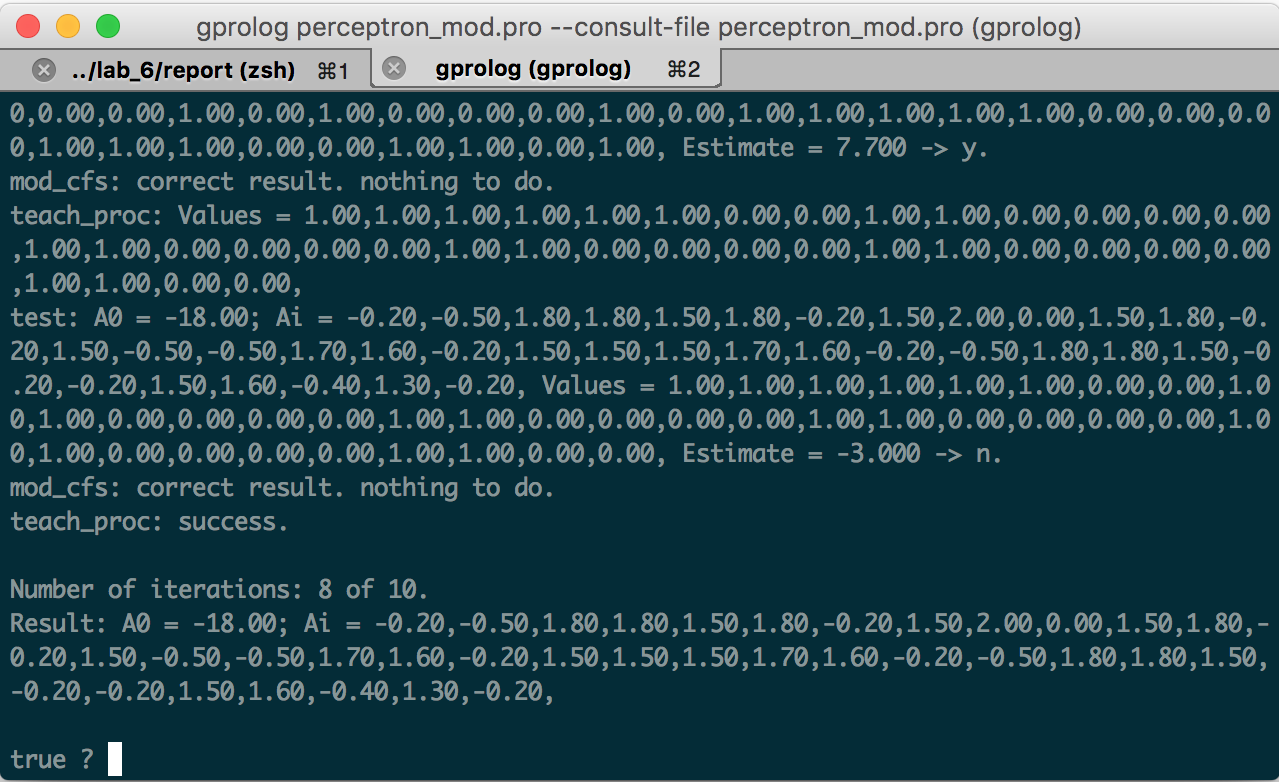
\includegraphics[width=130mm]{img/results}
  \caption{Результат работы программы}
  \label{fig:results}
\end{figure}

Исходный код программы расположен в приложении~А.

\newpage